\documentclass[]{scrartcl}

\usepackage[utf8]{inputenc}
\usepackage[T1]{fontenc}
\usepackage{lmodern}
\usepackage[ngerman]{babel}
\usepackage{amsmath}
\usepackage{listings}
\usepackage{graphicx}
\usepackage{float}
\usepackage{hyperref}

\usepackage{color}

%% Commands
\newcommand{\n}{\newline}

\title{Quality Messurements}
\subtitle{King of Jawa}
\author{Pascal Bürklin, Isabel Geissmann, Jannik Jaberg, Nikolai Rutz}
\date{\today}
\begin{document}
\maketitle
\begin{figure}[H]
	
\includegraphics[width=\linewidth]{LOGO.png}
\end{figure}
\tableofcontents

\section{Richtigkeit}
\label{sec:Richtigkeit}
\textbf{Ziel:} Um die Richtigkeit von King of Jawa zu garantieren setzen wir uns als Ziel keine ‘ungenauen’ Berechnungen zu machen. Weiter sollen Rechenschritte in ihre eigenen Methoden ausgelagert werden um zu vermeiden dass lange Berechnungen den Aufnahmerahmen eines Developers zu sprengen. Messbar machen wir dies mittels dem Mantis-Bugtracker, welchen Pascal auf seiner Website aufgesetzt hat. Uns ist es wichtig dass wir jeden Bug bis zu seinem gesetzten Due-Date fixen oder zumindest bearbeiten. Bei gravierenden Bugs wollen wir höchstens 2 Tage warten bis zum Fix. \n
\textbf{Resultat:} Ungenaue Berechnungen wurden alle behoben und die Verwendung des Bugrackers wird im Punkt \hyperref[ssec:Bugs]{Bugs und Bug Tracker} beschrieben.\n
\textbf{Fazit: PASSED}
\section{Angemessenheit}
\textbf{Ziel:} Weiter ist die Angemessenheit ein wichtiger Punkt. Da manchmal eine Abschätzung, ob ein Algorithmus sinnvoll oder nicht ist, ist  für uns zu diesem Zeitpunkt noch schwierig, wollen wir dennoch dies als Nebenziel setzen, die Implementierten Algorithmen und/oder Datenstrukturen zu reflektieren und zu entscheiden, ob diese im entsprechenden Konsens angemessen sind. Was jedoch sinnvoll, machbar und konsequent messbar ist, ist Spaghetti-Code zu vermeiden. Deshalb haben wir uns dafür entschieden Methoden mit über 50 Zeilen in weitere Untermethoden abzukapseln. Dies sollte Verständlichkeit und Übersichtlichkeit stark fördern. Die Ausnahme bestätigt die Regel: Klar ist dies nicht zu 100\% umsetzbar - es gibt immer Ausnahmen wie beispielsweise run() Methoden, welche trotz über 50 Zeilen immer noch übersichtlich sein können. Deshalb setzen wir uns als Mass ungefähr 90\% der Methoden 50 Zeilen nicht überschreiten dürfen.\n
\textbf{Resultat:} Bezüglich der Angemessenheit haben wir uns richtig ins Zeug gelegt. Spaghetti-Code haben wir kaum mehr, da Pascal darauf bestanden hat nach jedem Milestone die Codebase zu refactoren und optimieren. Auch bei den Algorithmen und Datenstrukturen haben wir uns einiges überlegt. Anstelle von Listen haben wir in gewissen Fällen Hashtabels oder Maps benutzt. Bei der Länge der Methoden haben wir gemerkt, dass dies nichtt immer durchsetztbar ist. Bei den Resourcengebäudeleveln beispielsweise hat jede Klasse eine Level Methode, welche über 100 Zeilen lang ist, wie auch einige run() Methoden, die über 50 Zeilen lang sind.\n
\textbf{Fazit: FAILED}
\section{Sicherheit}
\textbf{Ziel:} Um Spass am Spiel zu garantieren ist die Sicherheit ein weiterer Kernpunkt den QAs. Messbar ist dies nicht wirklich, jedoch probieren wir allfällige Sicherheitslücken im Code, die durch Injection exploited werden können zu minimieren. Beispielsweise wird bei einer removeRequest für eine Lobby dir Socket des Owners und der Socket des Clients, der die Request gesendet hat, verglichen um sicherzugehen, dass nicht ein anderer Client Lobbies schliessen kann.\n
\textbf{Resultat:} Wie im Ziel erwähnt wollen wir möglichst viele Sicherheitslücken schliessen. Dies haben wir getan, sobald uns eine Lücke auffiehl, schlossen wir sie. Jedoch sind sicherlich nicht alle Lücken geschlossen und wir können auch keine Garantie geben, dass unser Spiel nicht hackable oder cheatable ist. Dennoch sind wir sehr zuversichtlich, dass wir Spielspass ohne Sicherheitslücken liefern können.\n
\textbf{Fazit: PASSED}
\section{Modifizierbarkeit}
\textbf{Ziel:} Da die Spielidee von King of Jawa beliebig erweiterbar ist,  setzen wir uns als weiteres Kernmerkmal die Modifizierbarkeit. Dem haben wir mit unserem Kommunikationsprotokoll bereits  einen fundamentalen Grundbaustein gesetzt. Mit Hilfe eines entity-component-system erreichen wir dies. Dies zu verwirklichen ist es ziemlich einfach, nämlich wir haben ein Entity-Component-System oder nicht. Wenn wir diese Bedingungen alle berücksichtigen, sollten Änderungen an Gebäuden oder hinzugefügen neuere Gebäude sehr einfach sein. \n
\textbf{Resultat:} Das Systen wurde im Verlauf des Projekts drei Mal refactored und verbessert. Mitlerweile ist es ziemlich einfach neue Gebäude zu implementieren und bestehenden Gebäuden Attribute zu geben. Dafür hat sich Nikolai ein Balancing-System überlegt und implementiet, dies unterstützt das Entity-Component-System extrem. So einfach wie wir uns dies vorgestellt haben ist es jedoch nicht. Man kann nicht einfach nur eine neue Klasse erstellen, sondern muss noch in vier weitern Klassen Anpassungen machen. \n
\textbf{Fazit: FAILED}
\section{Analysierbarkeit}
\textbf{Ziel:} Für die Analyse implementieren wir einen Bugtracker, wie bereits im Punkt \hyperref[sec:Richtigkeit]{Richtigkeit} beschrieben und einen Debugmode, für Client und Server.\n
\textbf{Resultat:} Mithilfe unseres Debugmodes und dem Bugtracker haben wir einen schnellen Weg geschaffen, Fehler in unserem Projekt zu finden und zu beheben. Auch die CI half uns oft Nullpointer zu erkennen und finden. Mitlerweile haben wir sogar ein ErrorLog File welches hilft Fehler zu analysieren und auszumertzen. Mehr dazu bei den Punkten \hyperref[ssec:Bugs]{Bugs und Bug Tracker} und \hyperref[ssec:CI]{CI}.\n
\textbf{Fazit: PASSED}

\section{Rahmenbedingungen}
\subsection{Bugs und Bug Tracker}
\label{ssec:Bugs}
\textbf{Ziel:} Alle Bugs die auftreten werden in unserem Bugtracker festgehalten und gemäss Beschreibung im Ziel des Punkt \hyperref[sec:Richtigkeit]{Richtigkeit} bearbeitet.\n
\textbf{Resultat:} Wie bereits im QA beschrieben haben wir Mantis als Bug Tracker gewählt und diesen auch immer benutzt. Die im Milestone 3 angegebenen Fristen von 2 Tagen haben wir jedoch gesprengt. Es war uns nicht möglich jeden Bug so zu behandel. Deshalb entschieden wir uns um und setzten spezifische Due Dates für jeden Bug. Gravierende Bugs bearbeiteten wir immer innerhalb von 2 Tagen aber andere auch noch kurz vor knapp bis zum jeweiligen Meilenstein. 
\begin{figure}[H]
	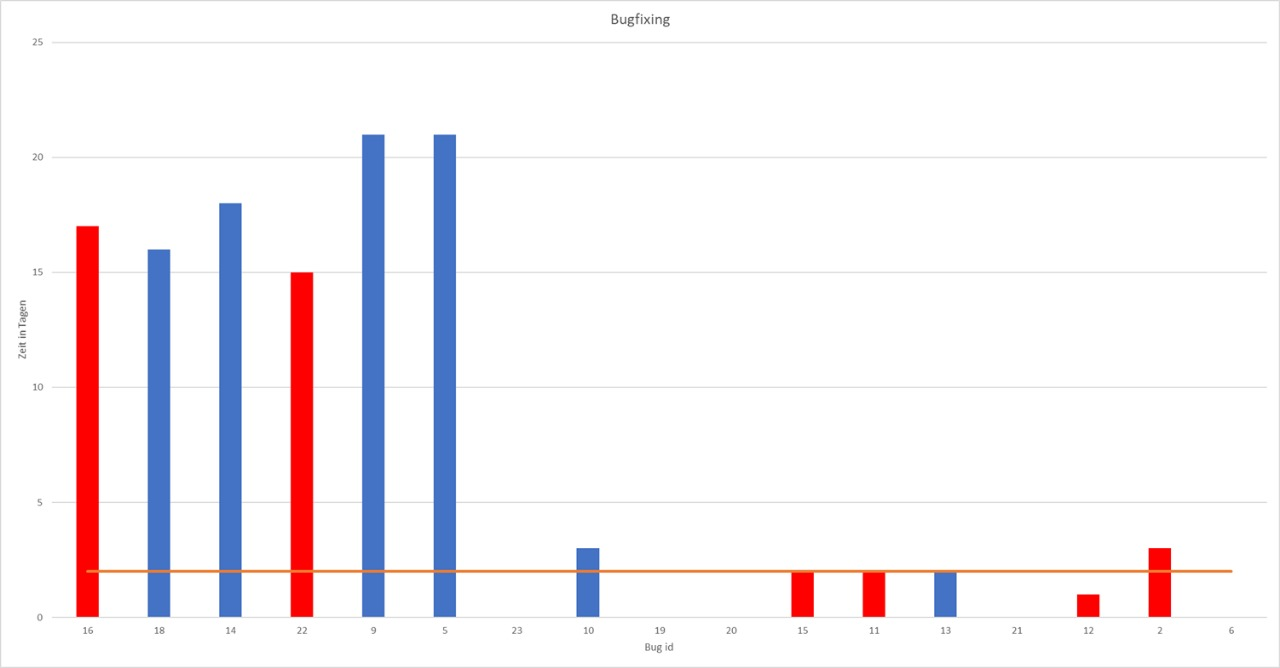
\includegraphics[width=\linewidth]{bugs/tabel.jpeg}
\end{figure}
Hier sieht man alle getrackten Bugs in Abhängigkeit zur Zeit in der sie behoben wurden. Rot sind hoch priorisierte Bugs mit Due Date von 2 Tagen. Die Blauen sind irgendwelche Bugs mit Due Date bis zum nächsten Meilenstein oder noch später. Wenn kein Balken vorhanden ist, wurde der Bug in unter 24h behoben. Also sind drei rote Bugs über ihr Due Date geschossen. Bei den Bugs mit der ID 16 und 22 war der Grund ganz simpel. Wir haben sie nicht geschlossen. Bug 2 ging uns effektiv durch die Lappen und wir versäumten sein Due Date. 
\begin{figure}[H]
	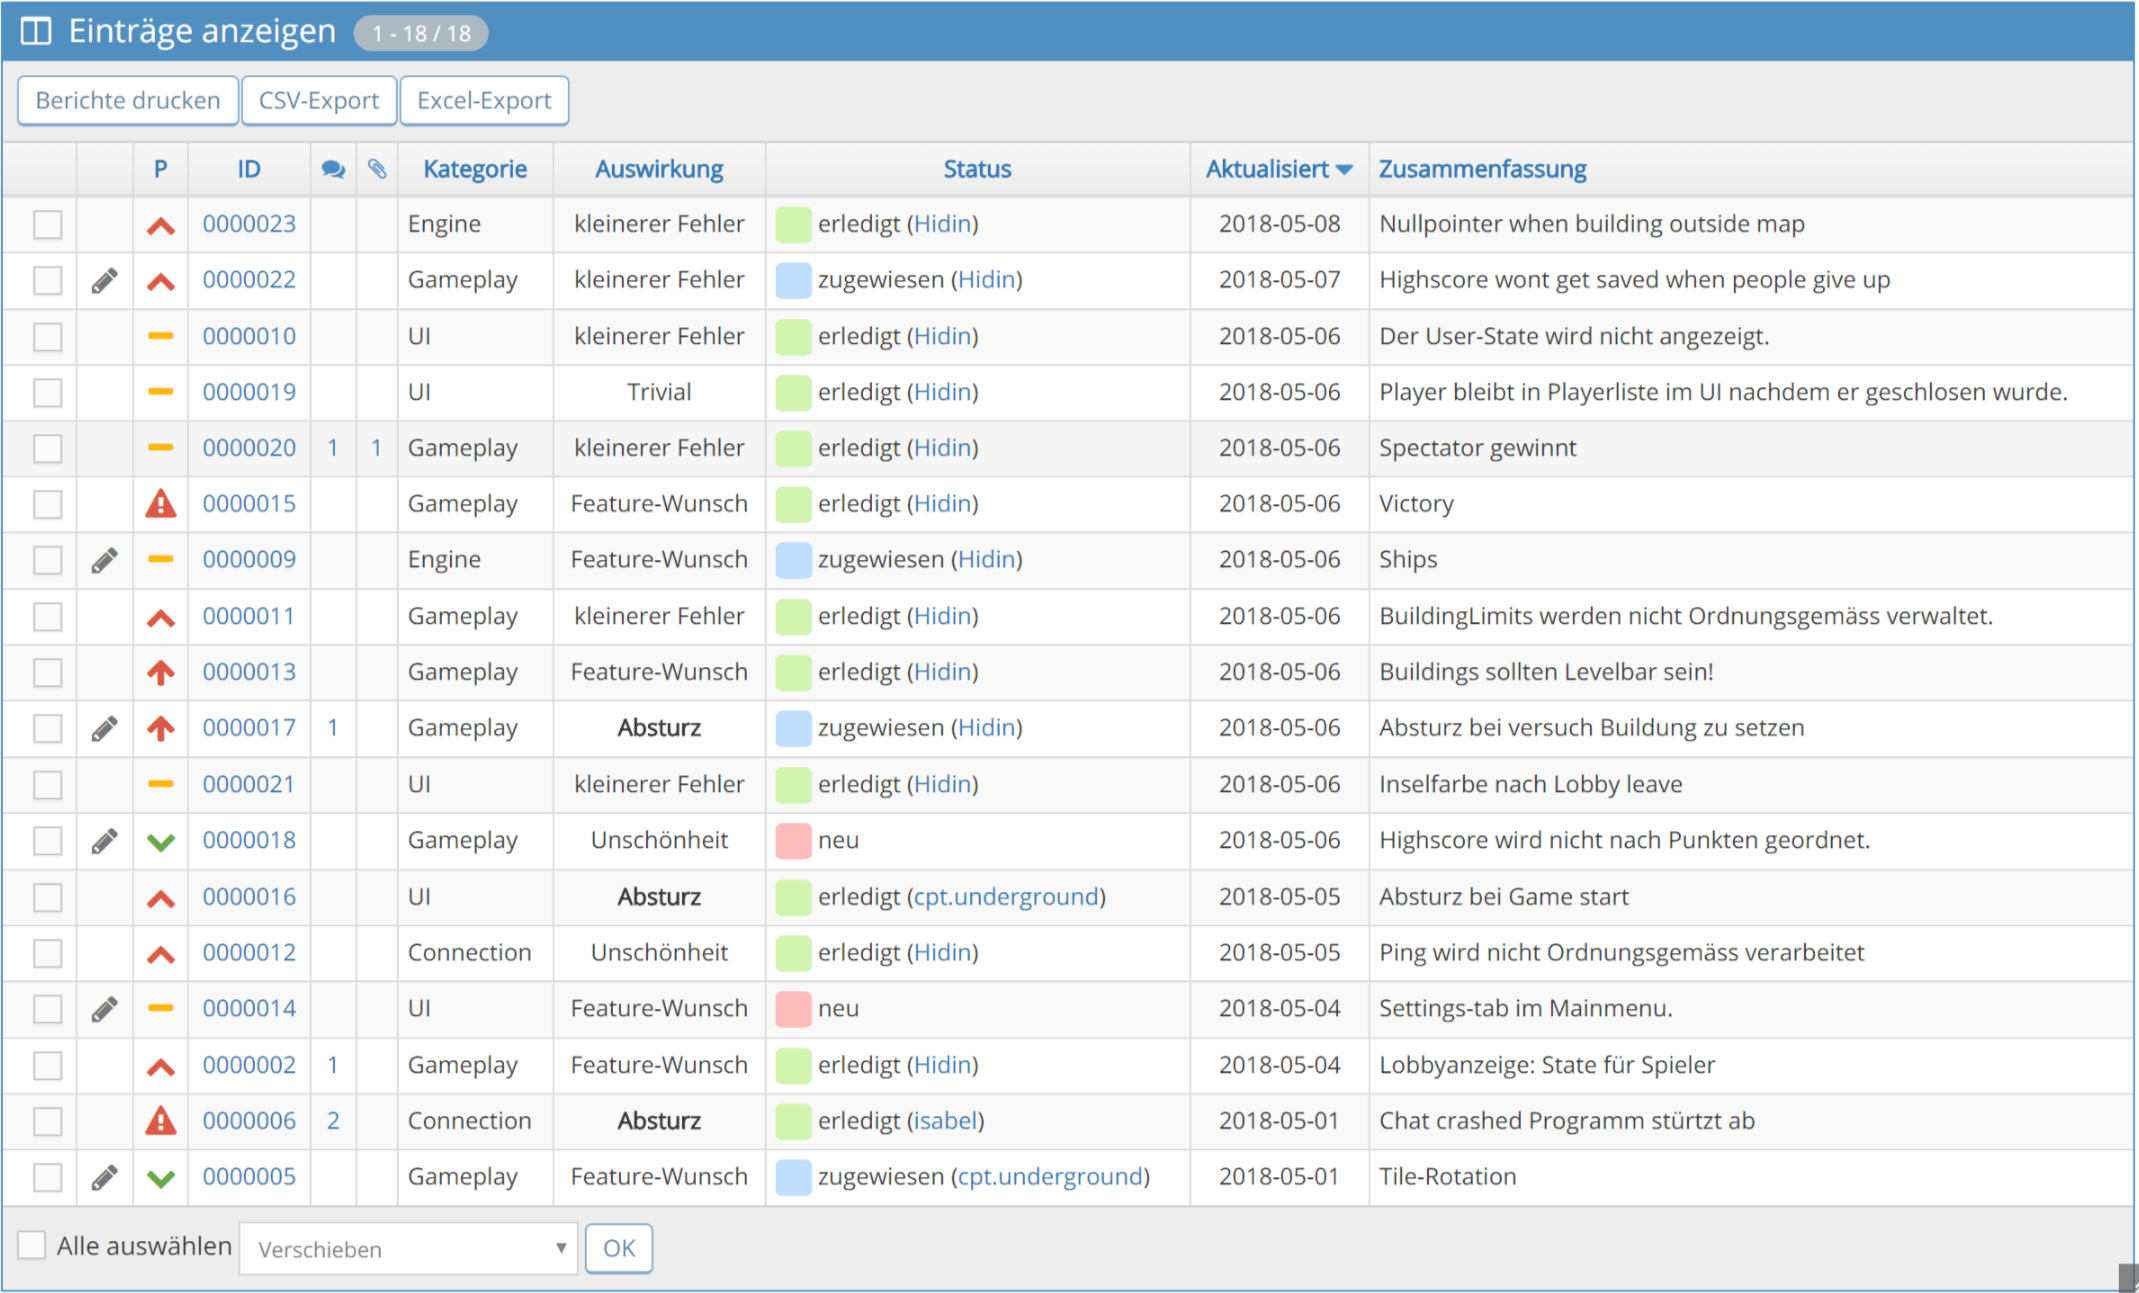
\includegraphics[width=\linewidth]{bugs/mantis.png}
\end{figure}
In diesem Bild sieht man alle Bugs die wir bis jetzt getrackt haben. An diesem Screenshot sieht man gut, dass es noch nicht bearbeitete Bugs gibt, wie beispielsweise den Feature-Wunsch für ein Settings Button im Menü mit der ID 0000014. Dieser ist zugewiesen und hat das Due Date bis zum Meilenstein 5, was man im nächsten Bild gut sieht.
\begin{figure}[H]
	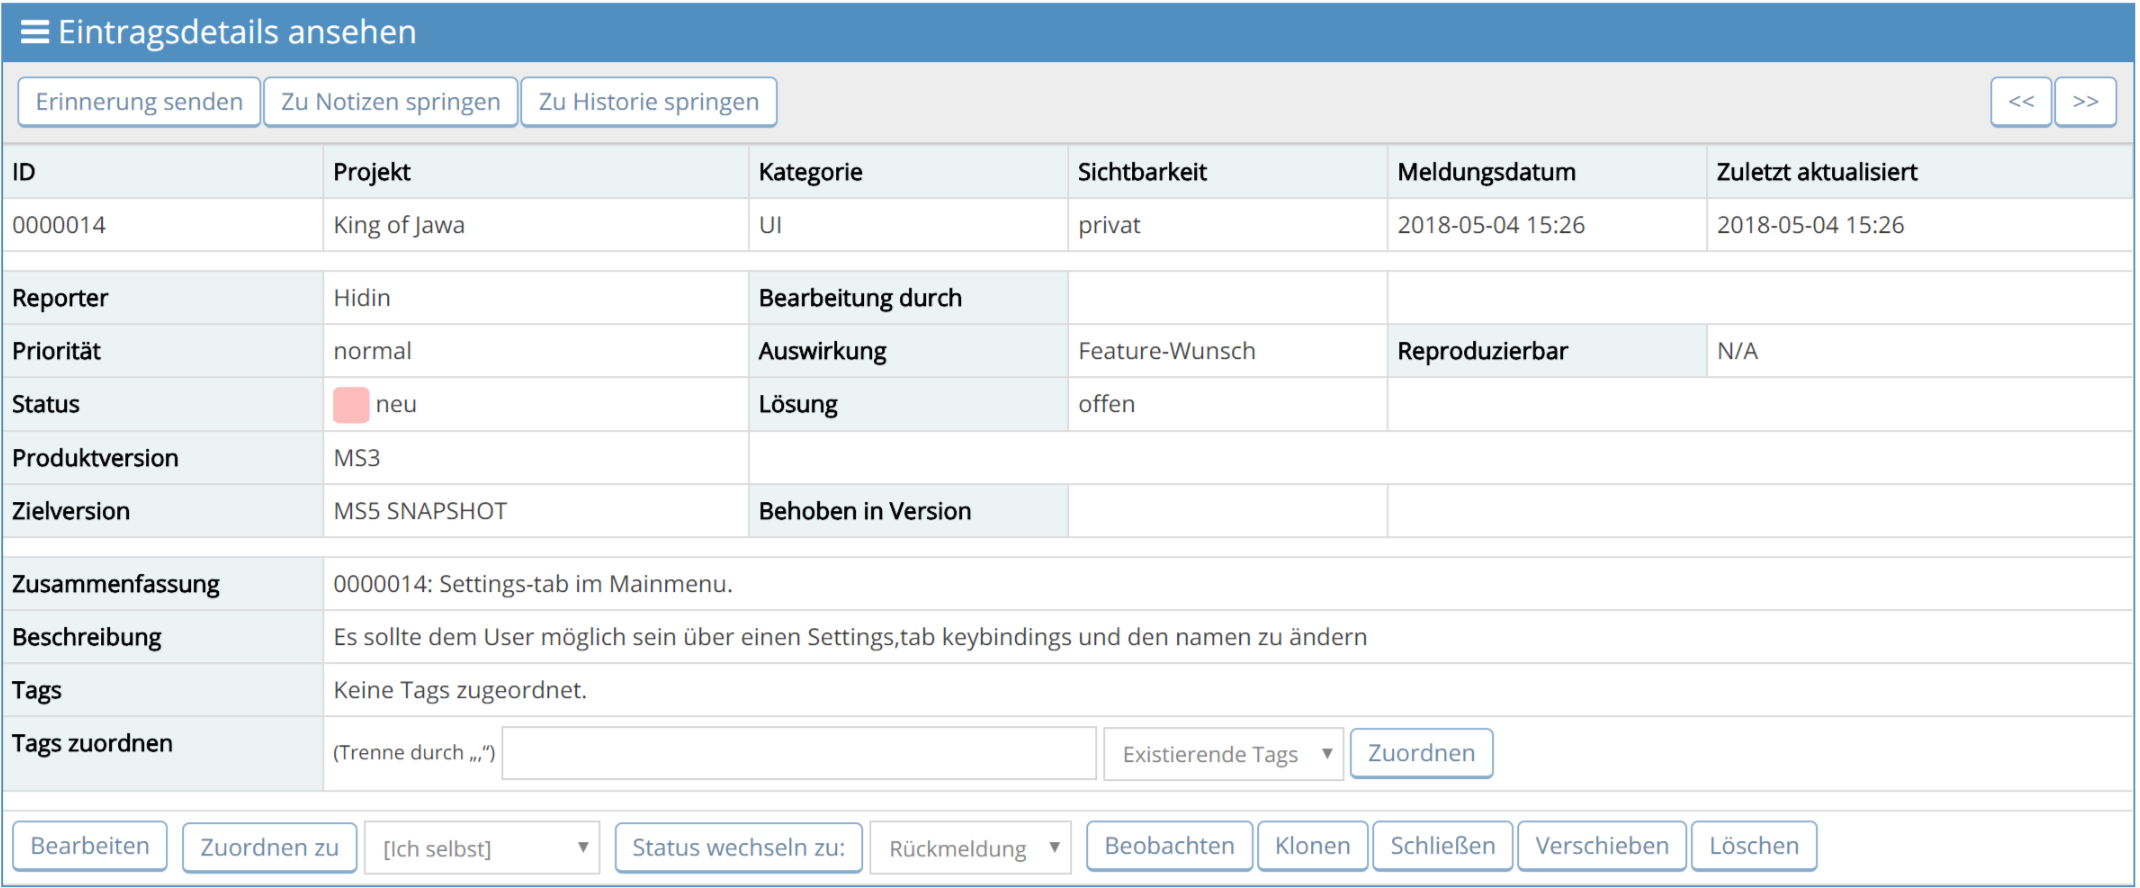
\includegraphics[width=\linewidth]{bugs/bug.png}
\end{figure}
Wie bereits gesagt könnten wir die Fristen nach dem Entscheid gut einhalten, was wir jedoch garnicht im Griff hatten war die Schliessung von Bugs (im nächsten Bild zusehen).
\begin{figure}[H]
	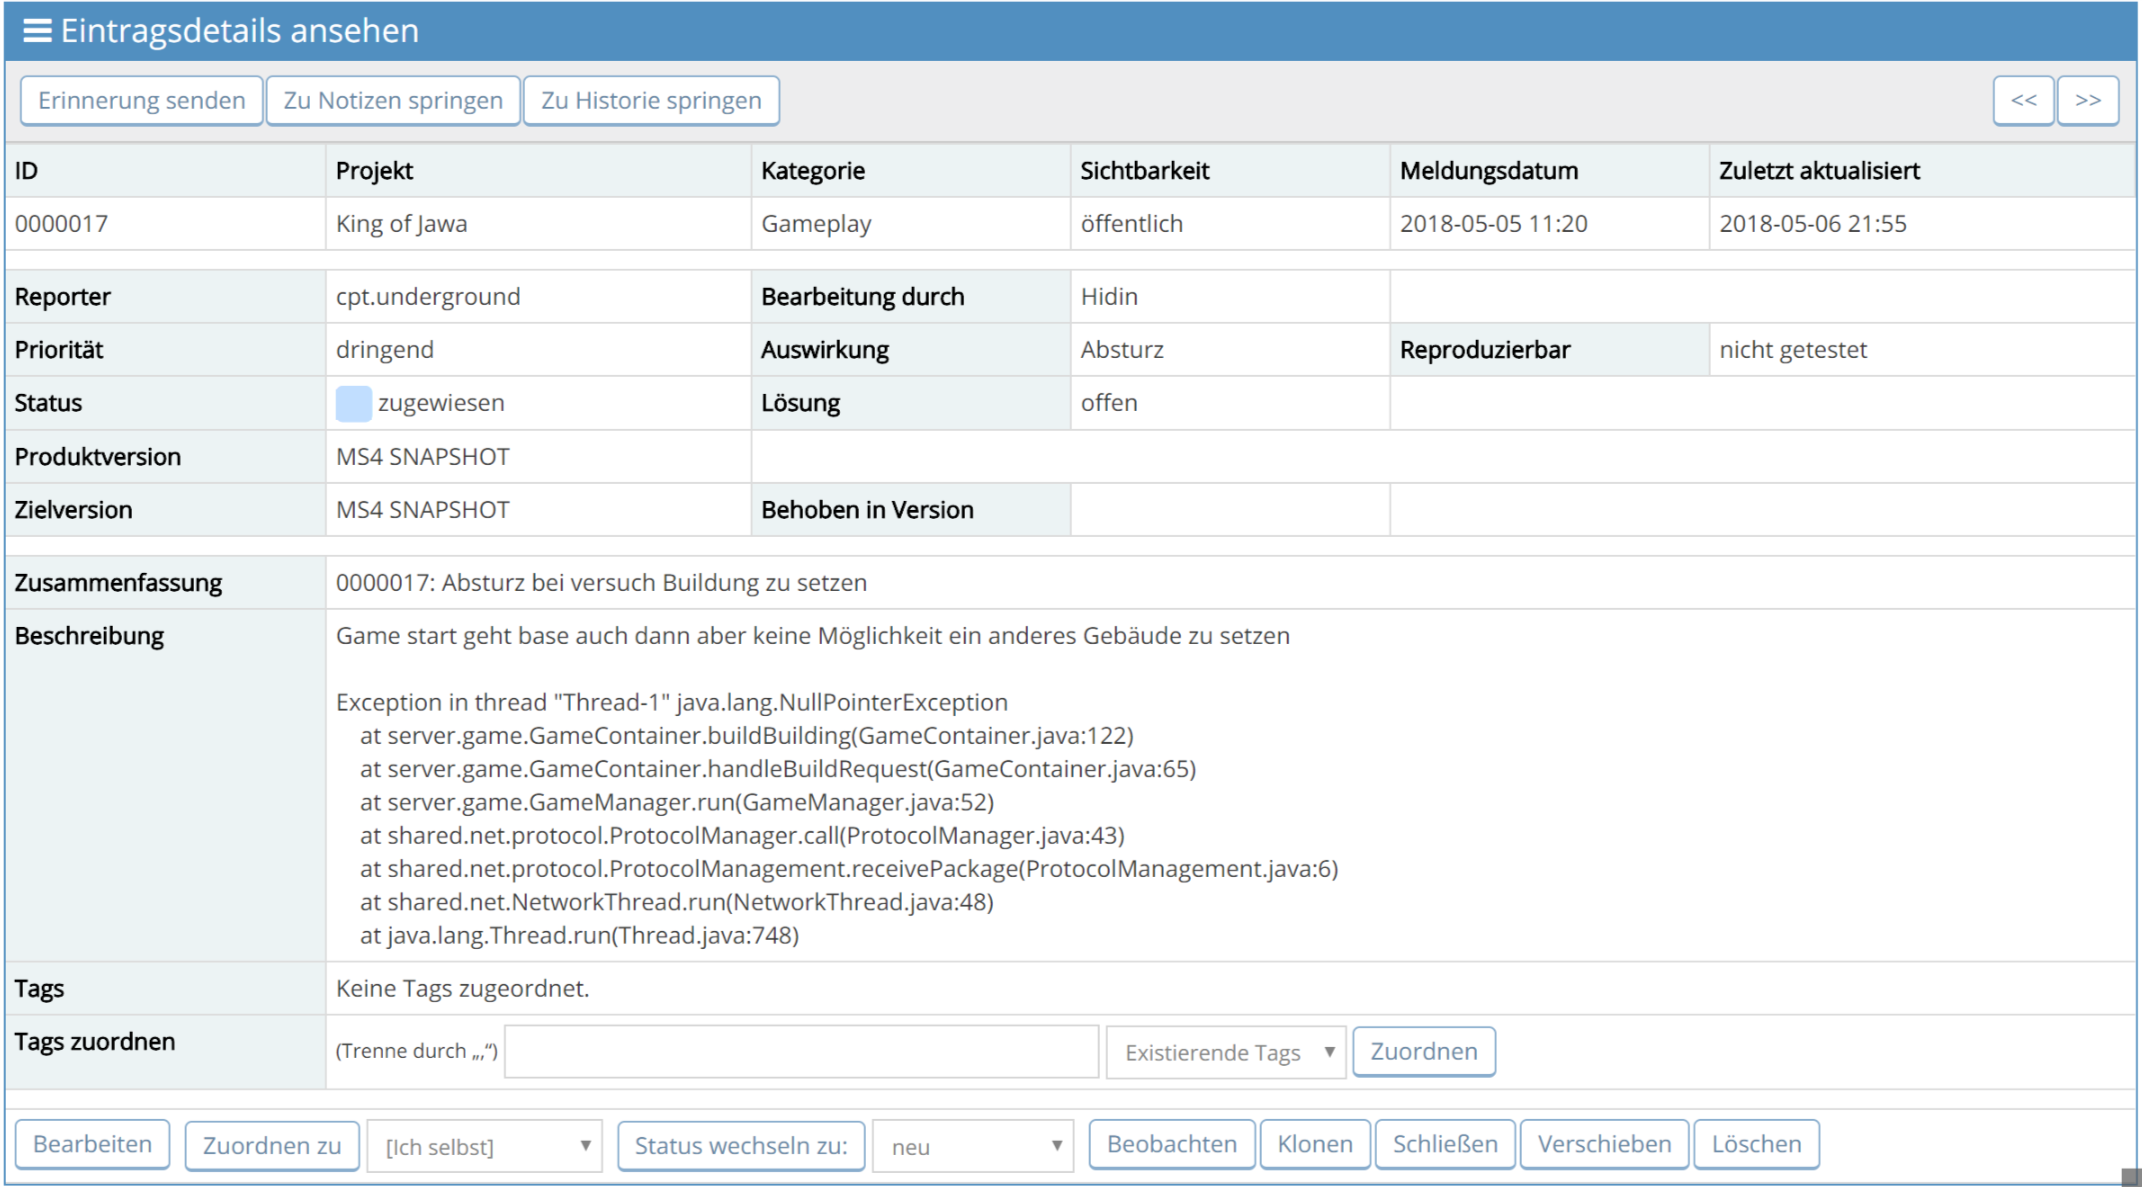
\includegraphics[width=\linewidth]{bugs/bug1.png}
\end{figure}
Hier handelt es sich um eine hoch priorisierten Bug, der zu einem Absturz führte. Der Bug war innert 2 Stunden behoben deutlich vor der angegebenen Zielversion für MS4. Er war aber offen bis zum 17. Mai 2018. Fazit dazu, wir hielten die Dates relativ gut ein doch haben das Bug Tracking Tool viel zu wenig benutzt. Viele Bugs kamen nicht einmal bis in den Bugtracker und andere wurden nur ineffizient eingetragen.\n
\textbf{Fazit: just PASSED}
\subsection{Unit Tests}
\textbf{Ziel:} Der Code wird fortlaufend mit Unit Tests überprüft.
Im Konzept einigten wir uns darauf ,dass jede Klasse die mehr als 100 Zeilen hat, mit Unit Tests überprüft werden muss. Alle Methoden dieser Klassen müssen mit Unit Tests abgedeckt werden. Nach dem Tutorat wurde uns jedoch klar, dass dies nicht umsetzbar ist. Daraufhin überlegten wir uns eine neue Messung. Entschieden haben wir uns dafür, dass wir wichtige Klassen testen. Dazu gehören:
\begin{itemize}
	\item Chain
	\item Serialization
	\item Package
	\item PackageManager
	\item User
	\item Session
\end{itemize} 
\textbf{Resultat:} 
Wir haben Jacoco zum Projekt hinzugefügt, um die Code Coverage zu betrachten. Momentan (Stand: 17. Mai 2018) liegt die Coverage der wichtigen Klassen wiefolgt.
\begin{figure}[H]
	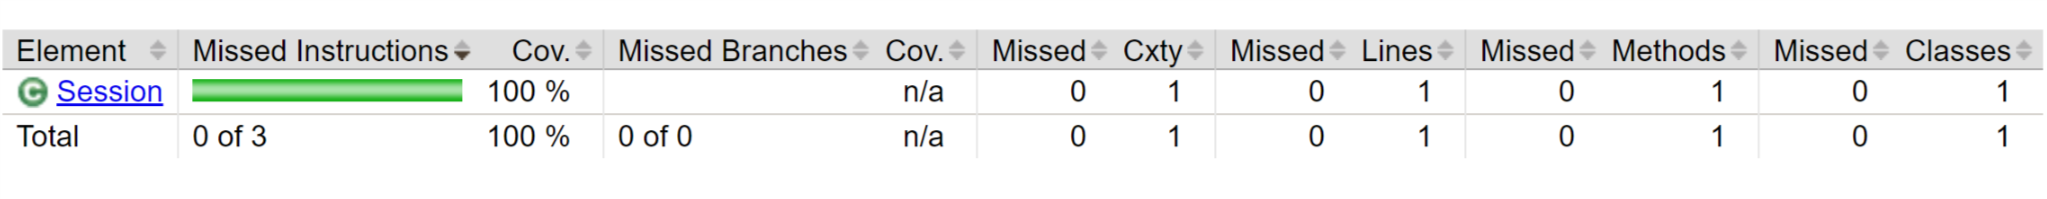
\includegraphics[width=\linewidth]{coverage/session.png}
	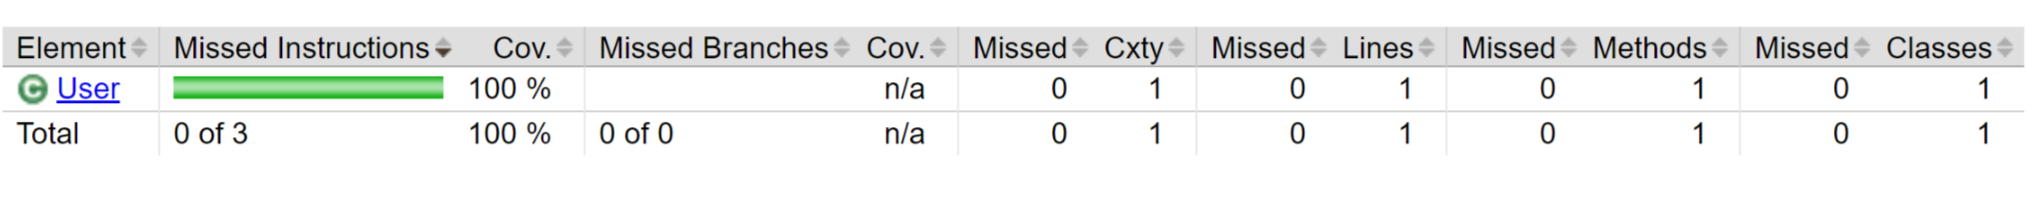
\includegraphics[width=\linewidth]{coverage/user.png}
	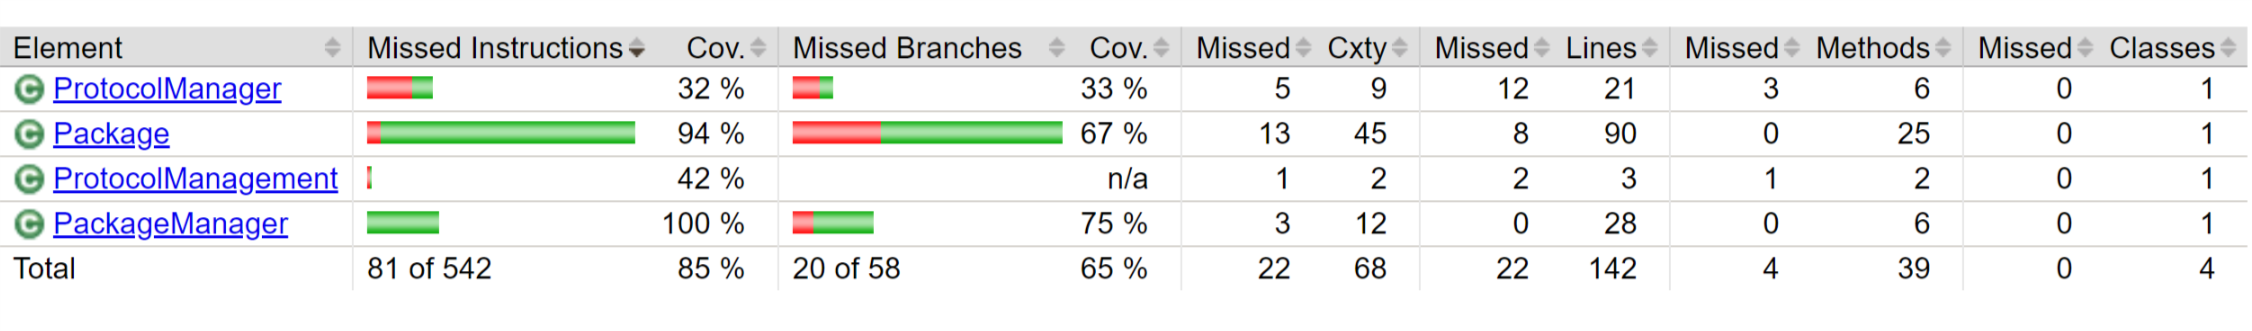
\includegraphics[width=\linewidth]{coverage/package.png}
	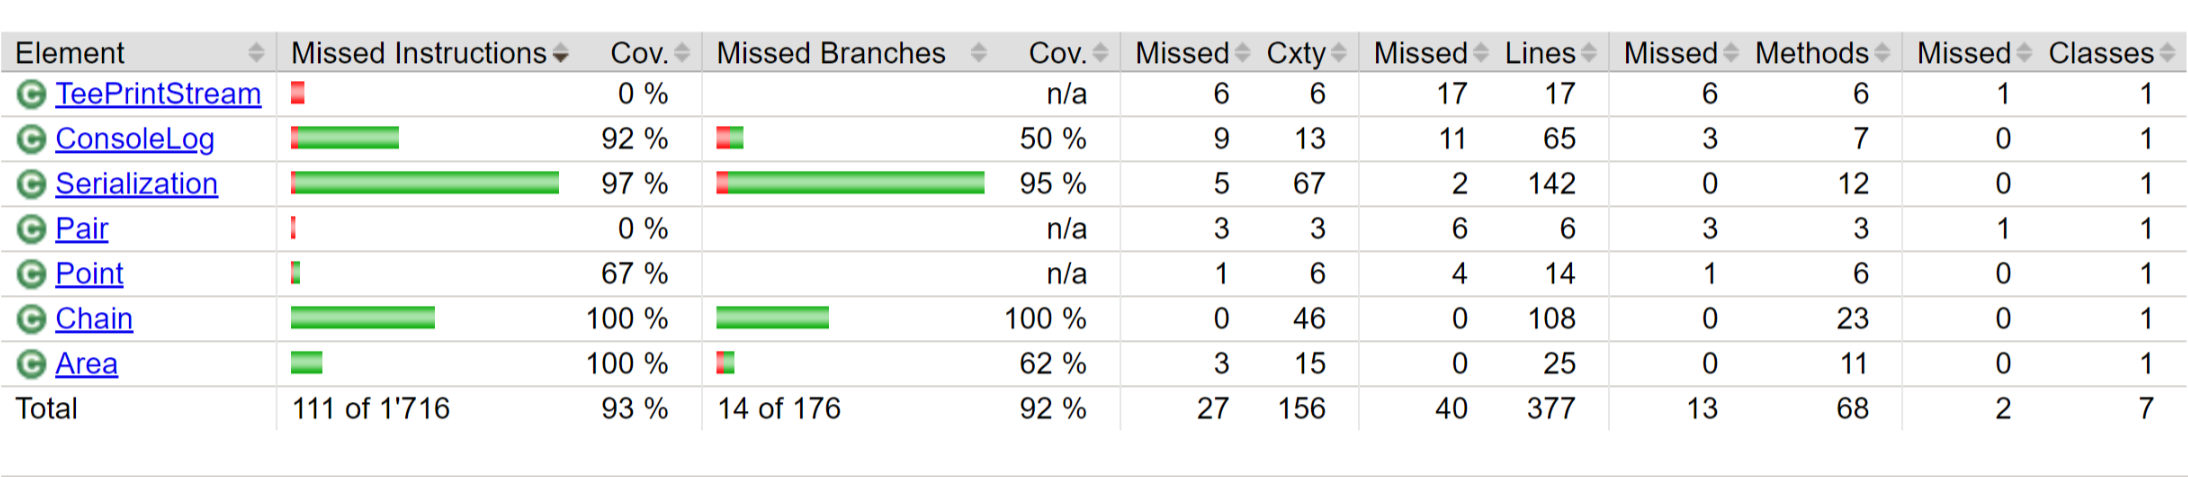
\includegraphics[width=\linewidth]{coverage/util.png}
\end{figure}
Hier auch noch eine Übersicht zur Overall Coverage Stand: 17. Mai 2018
\begin{figure}[H]
	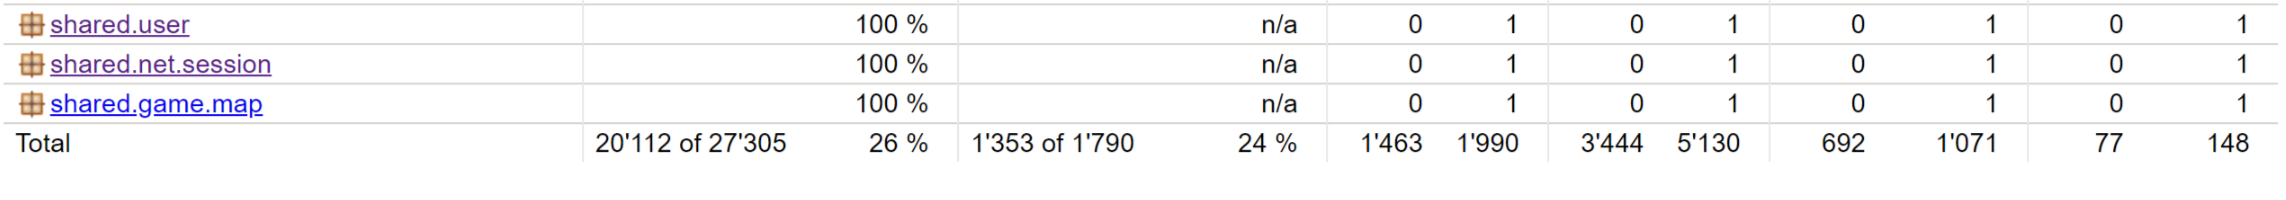
\includegraphics[width=\linewidth]{coverage/overall4.png}
\end{figure}
Bezüglich den UnitTests muss man sagen es war für alle von uns neu und wir hatten mühe damit. Meistens haben wir die UnitTests erst ganz am Schluss eines Features programmiert. Oder auch wurden Klasses die seit Milestone 2 stehen erst auf Milestone 4 getestet. Dies könnte man noch stark verbessern oder sogar mit TDD durchführen.
\textbf{Fazit: just PASSED}
\subsection{Playtesting}
\textbf{Ziel:} King of Jawa wird durch eine Testgruppe von 10 Personen getestet. Dafür wird ein Debug Modus implementiert. Dies gibt uns die Möglichkeit die Fehler einfacher nachzustellen um sie danach zu beheben.\n
\textbf{Resultat:} Unser Playtesting haben wir uns etwas anders vorgestellt. Wir haben extra einen Download zur Verfügung gestellt und einen Server auf den man sich mit dem Client verbinden kann. Doch ist uns aufgefallen, dass die Mitstudierenden alle eigene Probleme haben mit ihrem Projekt und die Kollegen von Pascal sich auch nicht wirklich darum gerissen haben unser Spiel zutesten. Deshalb blieb die meiste Arbeit des testing bei uns hängen.\n
\textbf{Fazit: FAILED}
\subsection{CI}
\label{ssec:CI}
\textbf{Ziel: } Die Benützung von CI.\n
\textbf{Resultat:} Das CI Tool in Git hat uns geholfen Fehler zu entdenken, die bei unseren Maschinen nicht aufgetretten sind. Bemerkt haben wir dies durch Marco. Bei ihm lief das buildscript bei der Abgabe von Milestone 4 nicht durch. Mithilfe der CI haben wir den Fehler finden und behenben können.\n
\textbf{Fazit: PASSED}
\subsection{Restliche Rahmenbedingungen}
\begin{itemize}
	\item JavaDoc \n
	JavaDocs haben wir immer geschrieben und gebuildet. Punkte gab es dafür auch immer, deshalb nehmen wir an, dass dies Genügend war. Für die Zukunft sollten alle von uns immer direkt nach der Implementation eines Features die JavaDocs schreiben und nicht erst am Schluss. Weiter könnten die Kommentare etwas ausführlicher sein.\n
	\textbf{Fazit: PASSED}
	\item Style Conventions \n
	Dies einzuhalten war nicht besonders schwer, da Intellij einem unter die Arme greift.\n
	\textbf{Fazit: PASSED}
	\item Name Conventions \n
	Name Conventions haben wir, in Anbetracht ein paar kleinen Ausreissern, immer angepasst.\n
	\textbf{Fazit: PASSED}
	\item Log4J \n
	Log4J haben wir aktiv benutzt, um zum Beispiel ein ErrorLog File zugenerieren, was die analyse von Fehlern, Bugs und Exceptions enorm vereinfachte. \n
	\textbf{Fazit: PASSED}
\end{itemize}
\end{document}